%!TEX root = ../dokumentation.tex

%TODO: Einleitungen überarbeiten
\chapter{Konzept}\label{cha:Konzept}
\section{Übersicht}\label{sec:Übersicht}
Die Anwendung besteht aus zwei verschiedenen Teilen, die beide mittels Docker deployt werden. 
Der eine Teil beinhaltet die Chat-Anwendung und die Spiellogik, der andere beinhaltet eine MongoDB, welche zum Speichern der Benutzer-Login-Informationen verwendet wird. 

\begin{figure}[H]
\centering
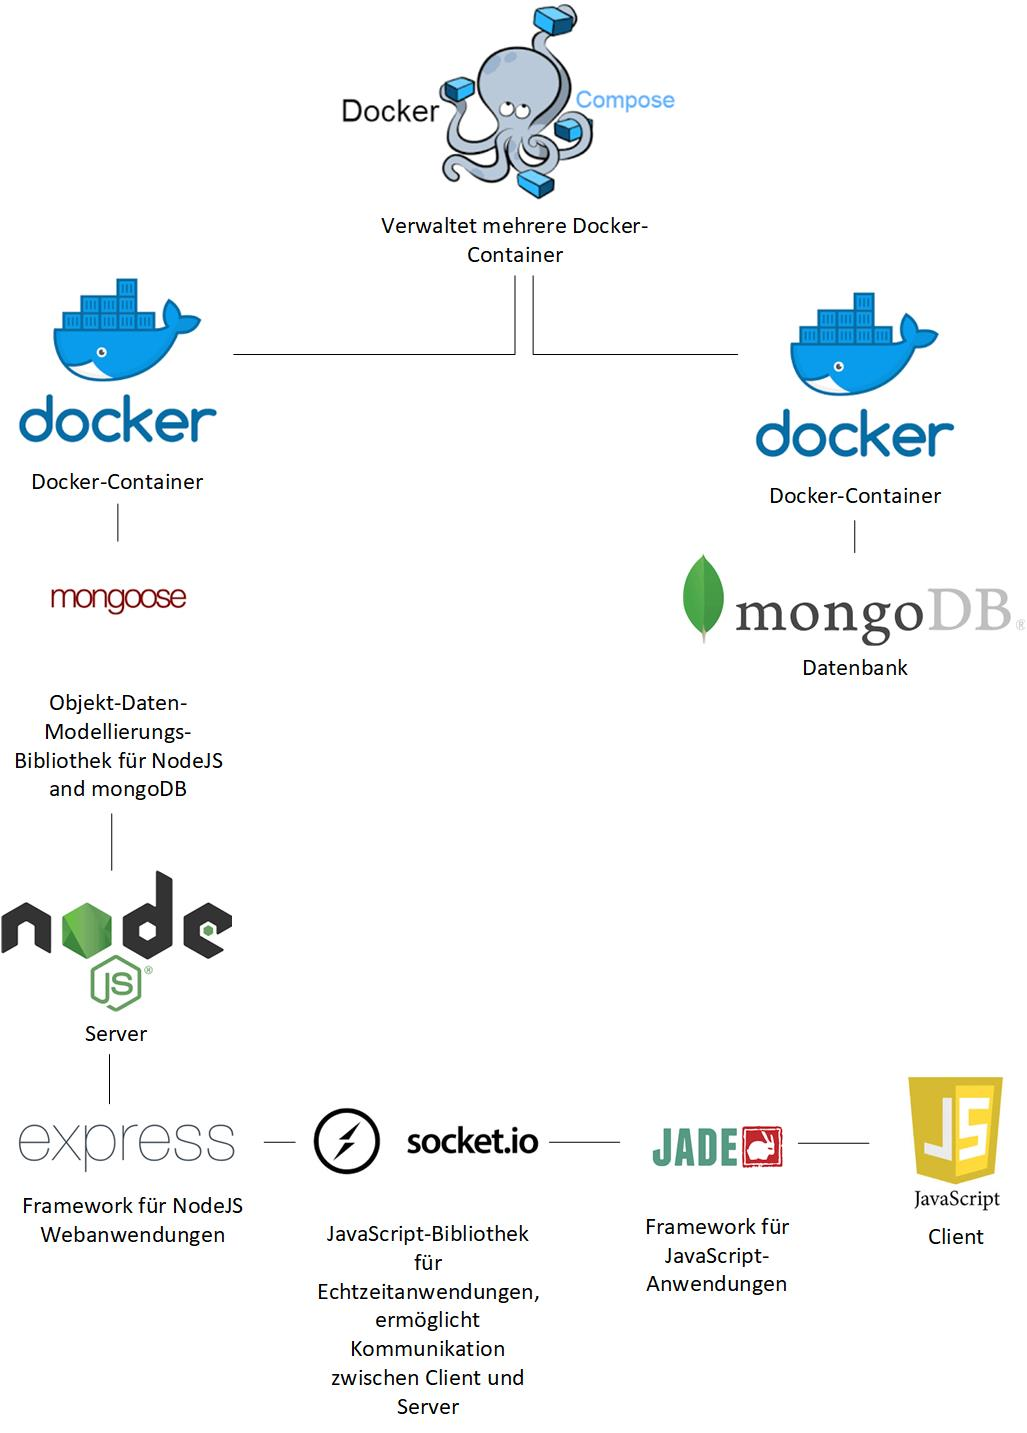
\includegraphics[width=0.75\textwidth]{images/uebersicht.jpg}
\caption{Übersicht der Anwendung}
\end{figure}


\section{Login und Registrierung}\label{sec:Login}
Beim Login hat der User die Möglichkeit haben, sich zu registrieren oder sich direkt einzuloggen. 

\section{Spiel}\label{sec:Spiel}

\section{Nachrichtenfilterung}\label{sec:Nachrichtenfilter}
Typischerweise werden bei einer Websocket-Anwendung allen Usern die eintreffenden Nachrichten angezeigt. Um dieses zu umgehen und nur den am Spiel beteiligten Spielern Spiel-relevante Nachrichten anzuzeigen, enthält die Nachricht die Namen der beiden am Spiel beteiligten Parteien. So kann der Client ermitteln, ob er am Spiel beteiligt ist und die Nachricht dann anzeigt oder nicht und die Nachricht ignoriert. 

\section{Gleichzeitiges Spielen mehrerer Spieler}\label{sec:Multiplegames}
Um es mehreren Spielern zu ermöglichen, gleichzeitig zu spielen, wird eine zweidimensionales Array genutzt. In einer Dimension sind jeweils ein Spielbrett, die zwei Spieler und den Spieler, der aktuell an der Reihe ist. In der anderen Dimension die verschiedenen Spiele. Sobald ein Spiel beendet wurde, werden die Daten aus dem Array mit dem Wert null belegt. Wenn ein neues Spiel begonnen wird, wird das durch das Array iteriert und die erste Position, die frei ist (also den Wert null hat) genutzt. Wenn keine freie Position gefunden werden konnte, wird ein neues Array erschaffen und angefügt. 

